% ANCHOR-FIG1

\begin{figure*}[t]
\centering
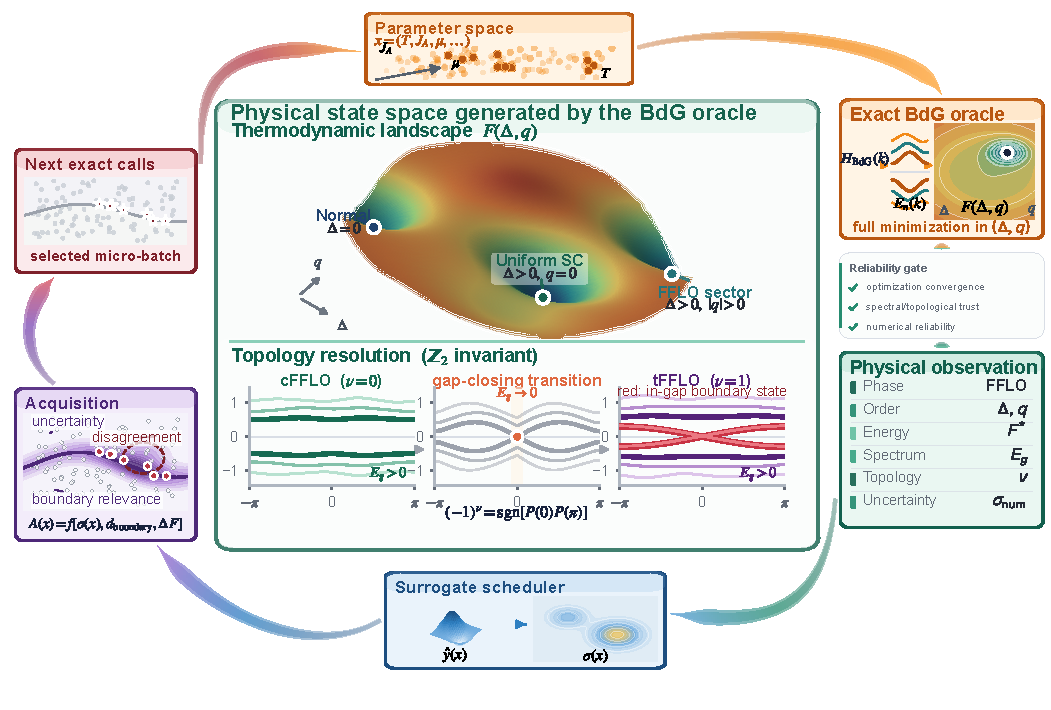
\includegraphics[width=0.96\textwidth]{figures/Fig1_candidate.pdf}
\caption{\textbf{Reliability-aware exact-oracle and active-learning hierarchy.} The central schematic organizes the physical state space generated by the BdG oracle: representative minima of $F(\Delta,q)$ encode Normal ($\Delta=0$), uniform-SC ($\Delta>0,q=0$), and FFLO ($\Delta>0,|q|>0$) sectors. Below, trusted gapped FFLO spectra distinguish cFFLO ($\nu=0$), a bulk-gap-closing transition, and reopened gapped tFFLO ($\nu=1$); the red crossing branch is an in-gap boundary state rather than a gapless bulk band. The right-hand oracle and reliability cards separate minimization, spectral/topological trust, and numerical status from the surrounding scheduler--acquisition cycle, which selects the next exact calls. All elements are schematic; the surrogate schedules BdG evaluations and does not determine physical labels or constitute convergence evidence.}
\label{fig:framework}
\end{figure*}

\textit{Exact oracle and physical labels.---}

For external coordinates $x=(k_BT/t,J_A/t,\mu/t,\ldots)$, the oracle uses the Nambu basis $\Psi_k=(c_{k+q/2,\uparrow},c_{k+q/2,\downarrow},\allowbreak c^\dagger_{-k+q/2,\uparrow},c^\dagger_{-k+q/2,\downarrow})^T$ and the block Hamiltonian

\begingroup\small\setlength{\arraycolsep}{3pt}\begin{equation}\label{eq:bdg}\begin{aligned}H_{\rm BdG}(k)&=\begin{pmatrix}h(k+q/2)-\mu&\Delta_q\\\Delta_q^*&-\sigma_yh^T(-k+q/2)\sigma_y+\mu\end{pmatrix},\\h(k)&=t\cos k+(0,\lambda_y\sin k,\lambda_z\sin k+J_A\cos k)\cdot\boldsymbol\sigma.\end{aligned}\end{equation}\endgroup

At every exact call it constructs $F(\Delta,q)$, refines competing minima, and accepts the lowest reliable state only after comparison with the normal reference. The frozen thresholds $\Delta_\epsilon=10^{-3}$ and $q_\epsilon=10^{-2}$ separate Normal, uniform-SC, and FFLO observations; phase labels remain distinct from trusted, boundary-ambiguous, and rerun-required numerical states. Edge minima trigger adaptive $q$-window expansion and shallow Normal--SC competition triggers local $\Delta$ refinement, while unresolved outcomes are withheld from clean physical training labels. Ensemble surrogates rank the next exact micro-batch from accepted observations; they are schedulers rather than physics solvers (Fig.~\ref{fig:framework}). Figure~\ref{fig:framework} is a schematic hierarchy and is not itself evidence that any convergence gate has closed.



\FloatBarrier

% ANCHOR-FIG2

\textit{Audited thermodynamic reconstruction.---}

The two-dimensional loop begins from 512 selected exact calls, with 506 labels retained in the frozen endpoint, and subsequently allocates calls around visible Normal/superconducting and uniform-SC/FFLO structure (Fig.~\ref{fig:thermo}). The acquisition combines phase uncertainty, boundary proximity, phase-facing regression uncertainty, numerical risk, and soft repulsion, but only returned BdG calculations enter the accepted dataset. The endpoint contains 7,434 exact observations: 1,867 Normal, 715 uniform-SC, and 4,852 FFLO labels. Its final phase-map change is 0.001629, the Normal--SC and uniform-SC--FFLO shifts are 0.004167 and 0, and trusted surprise is 0 for 127 trusted calls, satisfying the configured stopping rules. The separate 129-call hard-risk layer, including 19 coordinate matches retained in the trusted endpoint, is a numerical frontier rather than a fourth phase or evidence that uncertainty has been eliminated. The exact-sample map therefore supports an audited two-dimensional thermodynamic reconstruction under the registered criterion while retaining finite numerical risk (Fig.~\ref{fig:thermo}).

\begin{figure*}[t]
\centering
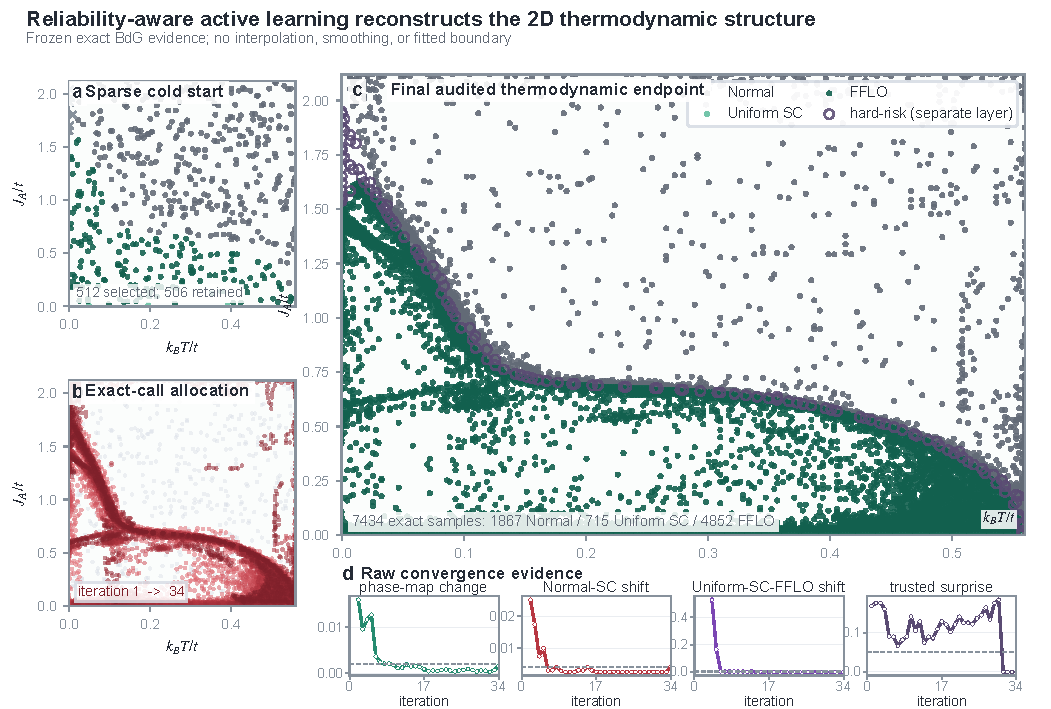
\includegraphics[width=0.96\textwidth]{figures/Fig2_candidate.pdf}
\caption{\textbf{Audited two-dimensional thermodynamic reconstruction.} \textbf{(a)} Sparse random-grid cold start with 512 selected exact calls; 506 retained frozen labels are shown. \textbf{(b)} Iteration-resolved exact-call allocation over $(k_BT/t,J_A/t)$ concentrates around visible thermodynamic structure. \textbf{(c)} Exact-sample endpoint with 7,434 observations: 1,867 Normal, 715 uniform SC, and 4,852 FFLO. Open rings denote the separate 129-call hard-risk numerical layer, not a phase. \textbf{(d)} Raw stopping observables at iteration 34: phase-map change 0.001629 (threshold 0.002), Normal--SC shift 0.004167 (threshold 0.004167), uniform-SC--FFLO shift 0, and trusted surprise 0 for 127 trusted calls (threshold 0.05). No interpolated field or fitted boundary is used, and finite numerical risk remains explicit.}
\label{fig:thermo}
\end{figure*}


\FloatBarrier

% ANCHOR-FIG3

\textit{Topology-resolved FFLO structure.---}

Topology is evaluated only after thermodynamic acceptance and only on trusted gapped FFLO observations. A full-Brillouin-zone minimum-gap guard and Pfaffians $P_0$ and $P_\pi$ determine the $\mathbb Z_2$ index away from their tolerances, assigning cFFLO for $\nu=0$ and tFFLO for $\nu=1$. Within the 4,345-point endpoint, 3,213 trusted gapped FFLO states divide into 2,290 cFFLO and 923 tFFLO observations and form a connected sampled structure (Fig.~\ref{fig:topology}). The support-restricted contour and local opposite-$\mathbb Z_2$ brackets diagnose a gap-closing transition; neither is an exact boundary, and the closing is not a stable third phase. The configured $k=8$ audit returns Decision A, with coverage $p_{95}=0.006185<0.00625$ and the remaining registered metrics passing. For the $k=6$ sensitivity setting, coverage $p_{95}=0.006269$ lies slightly above the same threshold, so the configured pass retains a neighborhood-size sensitivity and does not exhaust all refinements or nodal alternatives (Fig.~\ref{fig:topology}).

\begin{figure*}[t]
\centering
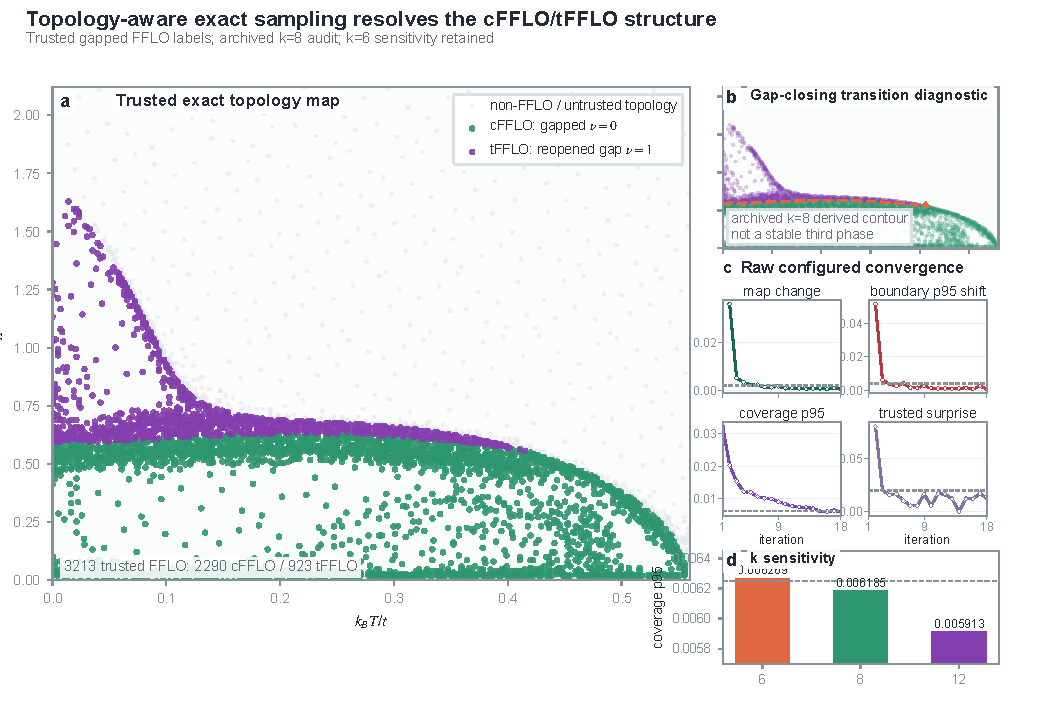
\includegraphics[width=0.96\textwidth]{figures/Fig3_candidate.pdf}
\caption{\textbf{Topology-resolved cFFLO/tFFLO discovery and configured audit.} \textbf{(a)} Trusted gapped FFLO subset of the 4,345-point exact endpoint: 3,213 states comprising 2,290 cFFLO ($\nu=0$) and 923 tFFLO ($\nu=1$) labels. \textbf{(b)} The archived support-restricted $k=8$ contour marks a gap-closing transition diagnostic; local opposite-$\mathbb{Z}_2$ brackets and the contour are supporting guides, not a stable phase or exact boundary. \textbf{(c)} Raw configured convergence histories for map change, boundary $p_{95}$ shift, coverage $p_{95}$, and trusted surprise. \textbf{(d)} The configured $k=8$ result gives Decision A with coverage $p_{95}=0.006185<0.00625$, whereas the $k=6$ sensitivity value $0.006269$ lies slightly above the same threshold. Topology is assigned from full-Brillouin-zone gap/Pfaffian evidence; the audit does not establish that every possible refinement or nodal alternative is exhausted.}
\label{fig:topology}
\end{figure*}

\begin{figure*}[t]
\centering
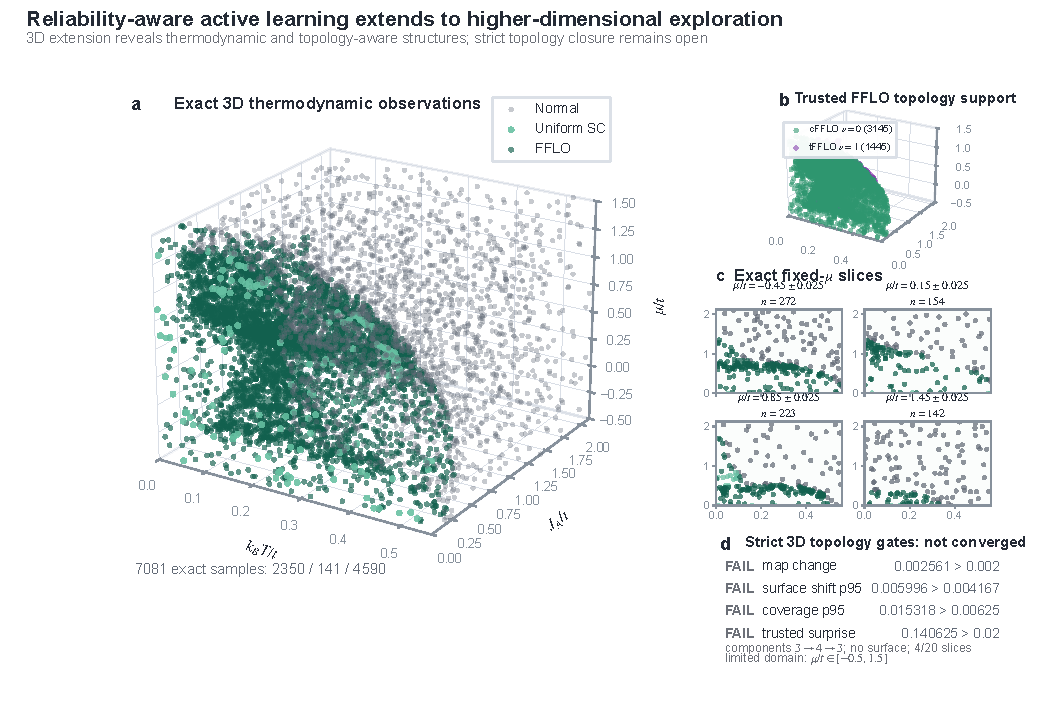
\includegraphics[width=0.96\textwidth]{figures/Fig4_candidate.pdf}
\caption{\textbf{Active-learning-enabled higher-dimensional exploration.} \textbf{(a)} Exact three-dimensional thermodynamic point cloud in $(k_BT/t,J_A/t,\mu/t)$ over $\mu/t\in[-0.5,1.5]$: 7,081 observations containing 2,350 Normal, 141 uniform-SC, and 4,590 FFLO states. \textbf{(b)} Trusted FFLO-only topology support comprises 3,145 cFFLO and 1,445 tFFLO points; no continuous topology surface is fitted. \textbf{(c)} Four explicit narrow fixed-$\mu$ bins, centered at $\mu/t=-0.45,0.15,0.85,$ and $1.45$ with half-width 0.025, show exact slice samples without interpolation between slices. \textbf{(d)} The final strict audit fails the registered map-change, surface-shift, coverage, trusted-surprise, and component-stability criteria. The 3D extension reveals thermodynamic and topology-aware structures across a finite sampled domain, but the strict three-dimensional topology convergence gates are not all closed and the discrete support does not imply a complete or continuous topology atlas.}
\label{fig:3d}
\end{figure*}


\FloatBarrier

% ANCHOR-FIG4

\textit{Higher-dimensional exploration.---}

The same oracle--scheduler separation extends the sampled coordinates to $x=(k_BT/t,J_A/t,\mu/t)$ over the finite interval $\mu/t\in[-0.5,1.5]$. The endpoint contains 7,081 exact observations: 2,350 Normal, 141 uniform-SC, and 4,590 FFLO states (Fig.~\ref{fig:3d}). Trusted FFLO-only topology support comprises 3,145 cFFLO and 1,445 tFFLO points and remains discrete rather than a fitted surface. Four explicit fixed-$\mu$ bins centered at $\mu/t=-0.45,0.15,0.85,$ and $1.45$, each with half-width 0.025, expose exact slice-to-slice structure without interpolation between slices. These point clouds and slices demonstrate higher-dimensional exploration that reveals thermodynamic and topology-aware structures across the sampled domain. The final strict audit nevertheless exceeds the registered map-change, surface-shift, coverage, and trusted-surprise thresholds, while component counts vary $3\to4\to3$. Thus the strict three-dimensional topology convergence gates are not all closed; visual continuity among slices is not a continuous topology surface, and the finite-domain result is not a complete three-dimensional atlas (Fig.~\ref{fig:3d}).

\FloatBarrier
